
% 
% Annual Cognitive Science Conference
% Sample LaTeX Paper -- Proceedings Format
% 

% Original : Ashwin Ram (ashwin@cc.gatech.edu)       04/01/1994
% Modified : Johanna Moore (jmoore@cs.pitt.edu)      03/17/1995
% Modified : David Noelle (noelle@ucsd.edu)          03/15/1996
% Modified : Pat Langley (langley@cs.stanford.edu)   01/26/1997
% Latex2e corrections by Ramin Charles Nakisa        01/28/1997 
% Modified : Tina Eliassi-Rad (eliassi@cs.wisc.edu)  01/31/1998
% Modified : Trisha Yannuzzi (trisha@ircs.upenn.edu) 12/28/1999 (in process)
% Modified : Mary Ellen Foster (M.E.Foster@ed.ac.uk) 12/11/2000
% Modified : Ken Forbus                              01/23/2004
% Modified : Eli M. Silk (esilk@pitt.edu)            05/24/2005
% Modified : Niels Taatgen (taatgen@cmu.edu)         10/24/2006
% Modified : David Noelle (dnoelle@ucmerced.edu)     11/19/2014

%% Change ''letterpaper'' in the following line to ''a4paper'' if you must.

\documentclass[10pt,letterpaper]{article}

\usepackage{cogsci}
\usepackage{pslatex}
\usepackage{apacite}
\usepackage{amsmath,amssymb}
\usepackage{graphicx}
\usepackage{color}
\usepackage{url}
\usepackage{todonotes}
\usepackage{mathtools}
\usepackage{stmaryrd}
\usepackage{booktabs}
\usepackage{array}

\newcommand{\den}[2][]{
\(
\left\llbracket\;\text{#2}\;\right\rrbracket^{#1}
\)
}

%\newcommand{\url}[1]{$#1$}


\definecolor{Blue}{RGB}{0,0,255}
\newcommand{\jd}[1]{\textcolor{Blue}{[jd: #1]}}  
\definecolor{Red}{RGB}{255,0,0}
\newcommand{\red}[1]{\textcolor{Red}{#1}}
\definecolor{Green}{RGB}{10,200,100}
\newcommand{\ndg}[1]{\textcolor{Green}{[ndg: #1]}}
\definecolor{Red}{RGB}{255,0,0}
\newcommand{\caroline}[1]{\textcolor{Red}{#1}}


 \newcommand{\denote}[1]{\mbox{ $[\![ #1 ]\!]$}}


\newcommand{\subsubsubsection}[1]{{\em #1}}
\newcommand{\eref}[1]{(\ref{#1})}
\newcommand{\tableref}[1]{Table \ref{#1}}
\newcommand{\figref}[1]{Fig.~\ref{#1}}
\newcommand{\appref}[1]{Appendix \ref{#1}}
\newcommand{\sectionref}[1]{Section \ref{#1}}

\title{Animal, dog, or dalmatian? Level of abstraction in nominal referring expressions}
%Animal, dog, or dalmatian? Contextual informativeness, utterance length and utterance frequency affect choice of referring expressions.

 
\author{{\large \bf Caroline Graf, Judith Degen, Robert X.D. Hawkins, Noah D.~Goodman} \\
  cgraf@uos.de, \{jdegen,rxdh,ngoodman\}@stanford.edu\\
  Department of Psychology, 450 Serra Mall \\
  Stanford, CA 94305 USA}



\begin{document}

\maketitle


\begin{abstract}


Nominal reference is very flexible---the same object may be called \emph{a dalmatian}, \emph{a dog}, or \emph{an animal} when all are literally true.
What accounts for the choices that speakers make in how they refer to objects?
The addition of modifiers (e.g.~\emph{big dog}) has been extensively explored in the literature, but fewer studies have explored the choice of noun, incuding its level of abstraction.
We collected freely produced referring expressions in a multi-player reference game experiment, where we manipulated the object's context.
We find that utterance choice is affected by the contextual informativeness of a description, its length and frequency, and the typicality of the object for that description.
Finally, we show how these factors naturally enter into a formal model of production within the Rational Speech-Acts framework, and that the resulting model predicts our quantitative production data.
%\red{The choice of referring expressions is highly context dependent. Whether speakers choose to refer to an object as a ``dalmatian'', a ``dog'', or an ``animal'' is determined partly by the features of the other objects present in the scene, as well as features of the utterance alternatives. In the first step, an exploratory analysis within a reference game setting demonstrates that speakers' choice of referring expression is dependent on a rich interplay of expressions' degree of contextual informativeness, their relative length combined with their relative frequency, as well as on the degree to which the referent is typical of a specific expression. If a competitor object of the same category (e.g., dog) as the target object is present in the display, speakers choose a more specific subcategory (e.g., ``dalmatian'') to refer to the target object. In contrast, when the competitor objects do not share the same (super-) category as the target, speakers are less constrained in choosing an appropriate referring expression. In this event, shorter expressions are preferred over longer ones, even more so when frequency of the expression is high. Moreover, the better the referent fits to the meaning of a referential expression due to being more typical of it, the more this expression is preferred. In a second step, quantitative effects are analyzed by a production model couched in the Rational Speech Act framework, which predicts the pattern of results by modelling a speaker as balancing an utterance's contextual informativeness with its cost relative to its alternatives while taking into account soft semantics of the meanings of expressions due to typicality effects.}
\textbf{Keywords:} 
referential expressions, levels of reference, basic levels, experimental pragmatics, computational pragmatics
\end{abstract}

%\section{\bf Introduction}

%Reference is ubiquitous in human communication. Unsurprisingly, a wealth of literature has been devoted to how speakers choose referring expressions from the many options available to them with the goal of distinguishing one object from its surroundings \red{cite cite cite deutsch pechmann sedivy gatt}. 
Referring to objects is a core function of human language, and a wealth of research has explored how speakers choose referring expressions \cite{herrmann1976, Pechmann1989, VanDeemter2012}.
However, most of this literature has focused on the addition of modifiers \cite<as in the choice between ``the dog'', ``the brown dog'', and ``the big brown dog'', e.g.,>{sedivy2003a, Koolen2011}. Here we investigate how speakers choose a simple nominal referring expression---what governs the choice of calling a particular object ``the dalmatian'', ``the dog'', or ``the animal'' when all are literally true? That is, what governs the choice of the taxonomic level at which an object is referred to?
Noun choice can be seen as the most basic decision in forming a referring expression.
Like modification, these choices differ in their specificity; unlike modification, the number of words used does not differ---in English, \emph{some} noun must be chosen.
In this paper we provide experimental evidence from a coordination game regarding the flexible choice of nominal referring expressions and explain this data with a probabilistic model of pragmatic production.

%they differs in that
%Given the taxonomic relations that hold between dalmatians, dogs, and animals, this choice shares with the choice between modified expressions that the three expressions differ in how much information about the intended referent is provided. Yet it differs in that the choice is not in adding additional adjectives, but in choosing between different nouns in the first place. The question is what governs this choice.


Previous evidence about the generation of referring expressions suggests that choice of reference level will depend on the interplay of several factors. 
Grice's Maxim of Quantity \cite{grice1975} implies a pressure for speakers to be sufficiently \emph{informative}.
For instance, a speaker who is trying to distinguish a dalmatian from a German Shepherd  would be expected to avoid the insufficiently specific term ``dog'' \cite{brennan1996}.
On the other hand, recent work in experimental pragmatics has shown that the choice of referring expression depends on the \emph{cost} of utterance alternatives \cite{rohde2012, degenfrankejaeger2013}; sometimes, speakers are willing to produce a cheap ambiguous utterance rather than a costly (e.g.~long or difficult-to-retrieve) unambiguous one. 
%That is, there is some evidence that speakers trade off an utterance's contextual informativeness and cost in systematic ways.
Finally, classic work on concepts suggests that \emph{typicality} of a referent within its category affects the choice of reference \cite{RoschEtAl76_BasicLevel}. In particular, speakers will generally choose to refer at the \emph{basic level} (e.g. ``dog''), but may become more specific for objects that are atypical for the basic level term.

%\todo[inline]{rdh: If we're going to touch on it at the end, I think we should say something here about how we're going to try to account for basic-level biases through these other factors, rather than building it in -- like ``how can we push around preferences for the basic level by manipulating context and cost?''}
%\caroline{I agree! I moved some things around and added a sentence on how we aimed to account for the bl bias by these factors }
%Finally, classic work on concepts has shown that objects within a category vary in \emph{typicality} \caroline{(cite Rosch's prototype theory from 1973?)}.


%Speakers do not always use basic level terms to refer. 
%
%In certain cases, the basic level does not suffice for unique reference, e.g., when the speaker is trying to distinguish a dalmatian from a German Shepherd. In this case, the pressure to be sufficiently informative \cite<as in the Maxim of Quantity,>{grice1975} overrides the preference for the basic level and speakers typically choose a subcategory level term \cite{brennan1996} \red{cite others before them}. 
%%In other cases, as a subcategory convention forms, speakers continue to refer at that level, despite not being necessary for unique reference \cite{brennan1996}.
%
%Informativeness and a preference for the basic level do not fully explain the variability in speakers' reference choices. Recent work in experimental pragmatics has shown that the choice of referring expression depends on its cost relative to alternative utterances \cite{rohde2012, degenfrankejaeger2013}; sometimes, speakers are willing to produce a cheap ambiguous utterance rather than a costly (e.g., long or difficult-to-retrieve) unambiguous one. That is, there is some evidence that speakers trade off an utterance's contextual informativeness and cost in systematic ways.

%\ndg{come back to the question of basic level in discussion, rather than intro?}

%%There is a well-documented preference for use of basic level terms (e.g., ``dog'' \red{cite}). 
%In a series of classic experiments on the structure of concepts, Rosch and colleagues established that there is a maximally informative level of abstraction in category taxonomies. Dogs have a large number of features in common---four legs, wagging tail, loyal companion----which differentiate them from other animals, but there are fewer features that distinguish dalmatians from German Shepherds. She called this level of abstraction (e.g.~``dog'') the \emph{basic level} \cite{RoschEtAl76_BasicLevel}. Importantly for us, participants in a free-response naming task were much more likely to use the basic level than the superordinate or subordinate level, even though they knew all three terms. 
%
%Finally, the picture is further complicated by \red{typicality effects that have also gone under the label of salience but nobody knows whether those are speaker-internal effects or audience design effects. refs in brennan \& clark, mitchell et al 2013, westerbeek et al 2015.} That is, speakers may sometimes add modifiers to a referring expression simply because the property denoted by the modifier is atypical of the referent, and hence, surprising. Conversely, speakers might sometimes use subcategory instead of basic level terms to refer to an object, if the object is not a very typical instance of the basic level. For example, a panda  bear might be a less typical bear than a grizzly bear, so speakers might prefer to refer to the panda as ``panda'' but to the grizzly as ``bear''.
%\jd{i don't know how much to foreshadow here about the utility of `overinformative' sub level use, because i don't know how the typicality model does; but this is the place to foreshadow that stuff, eg by reusing some of caroline and robert's prose commented out right after this.}

%Including more attributes than are necessary to identify a target object may at first seem to contradict the Maxim of Quantity by Grice (1975), namely to make one's contribution as informative than is required and not more, but what does it actually mean for an utterance to be more informative than *required*? Does it mean that this utterance mentions attributes redundantly irrespective of their utility? What if the so called ``redundant'' attributes (e.g. Arts, 2004; Arts, Maes, Jansen, \& Noordman, 2011) actually have an utility after all by influencing the processing of an utterance? Pechmann (1985) has argued that the excessive use of color adjectives in referential expressions does in fact contribute to the informativeness of the utterance, namely by excluding some (but not all) distractors. As a matter of fact, other studies have demonstrated that overspecified utterances give rise to shorter identification times compared to minimally specified expressions (Deutsch, 1976; Sonnenschein, 1982). Thus, ``overinformative'' behavior must not necessarily be irrational behavior. 


%A similar argument can be made for the the use of a level of reference less abstract than necessary for disambiguation and the dominance for the the basic level in the production of referential expressions. The basic level of reference, which Rosch et. al (1976) characterize as the level of abstraction at which the most basic category cuts are made, seems to have a special status in human categorization behavior: Basic level categoriy labels are not only the first labels used for categorization during perception of the environment, but also the labels which lead to fastest category verification. Basic levels also carry the most information and possess the highest category cue validity (compared with the sublevel ``dalmatian'' or superlevel ``animal''). Therefore it can be argued that being more specific than necessary has a positive effect on the processing of the utterance for the listener and thus ``overinformativeness'' contributes to the informativeness of the utterance.



%It is clear that the choice of level of reference depends on a rich interplay between at least the factors discussed in the previous paragraphs: the contextual informativeness of referring at that level, the utterance's cost (in terms of length and frequency), and the typicality of the referent's properties. What is unknown is how these different factors trade off, and indeed, how a speaker who tries to maximize the communicative efficiency of their utterances, \emph{should} trade off these different factors. 

To evaluate the impact of these factors on nominal reference we constructed a two-player online game (\figref{fig:procedure}). Participants saw a shared context of objects, one of which was indicated as the referent only to the speaker. The speaker was asked to communicate this object to the listener, who then chose among the objects. Critically, the speaker and listener communicated by free use of a chat window, allowing us to gather relatively natural referring expressions. We manipulated the category of distractor objects and used items that varied in utterance complexity and object typicality. This allowed us to evaluate whether each factor influences the referring expressions generated by participants. We expect that speakers will (1) tend to avoid longer or less frequent terms, and (2) will pragmatically prefer more specific referring expressions when the target and distractor(s) belong to the same higher-level taxonomic category or when distractors are more typical members of that category level.

\begin{figure}[tb]
\centering
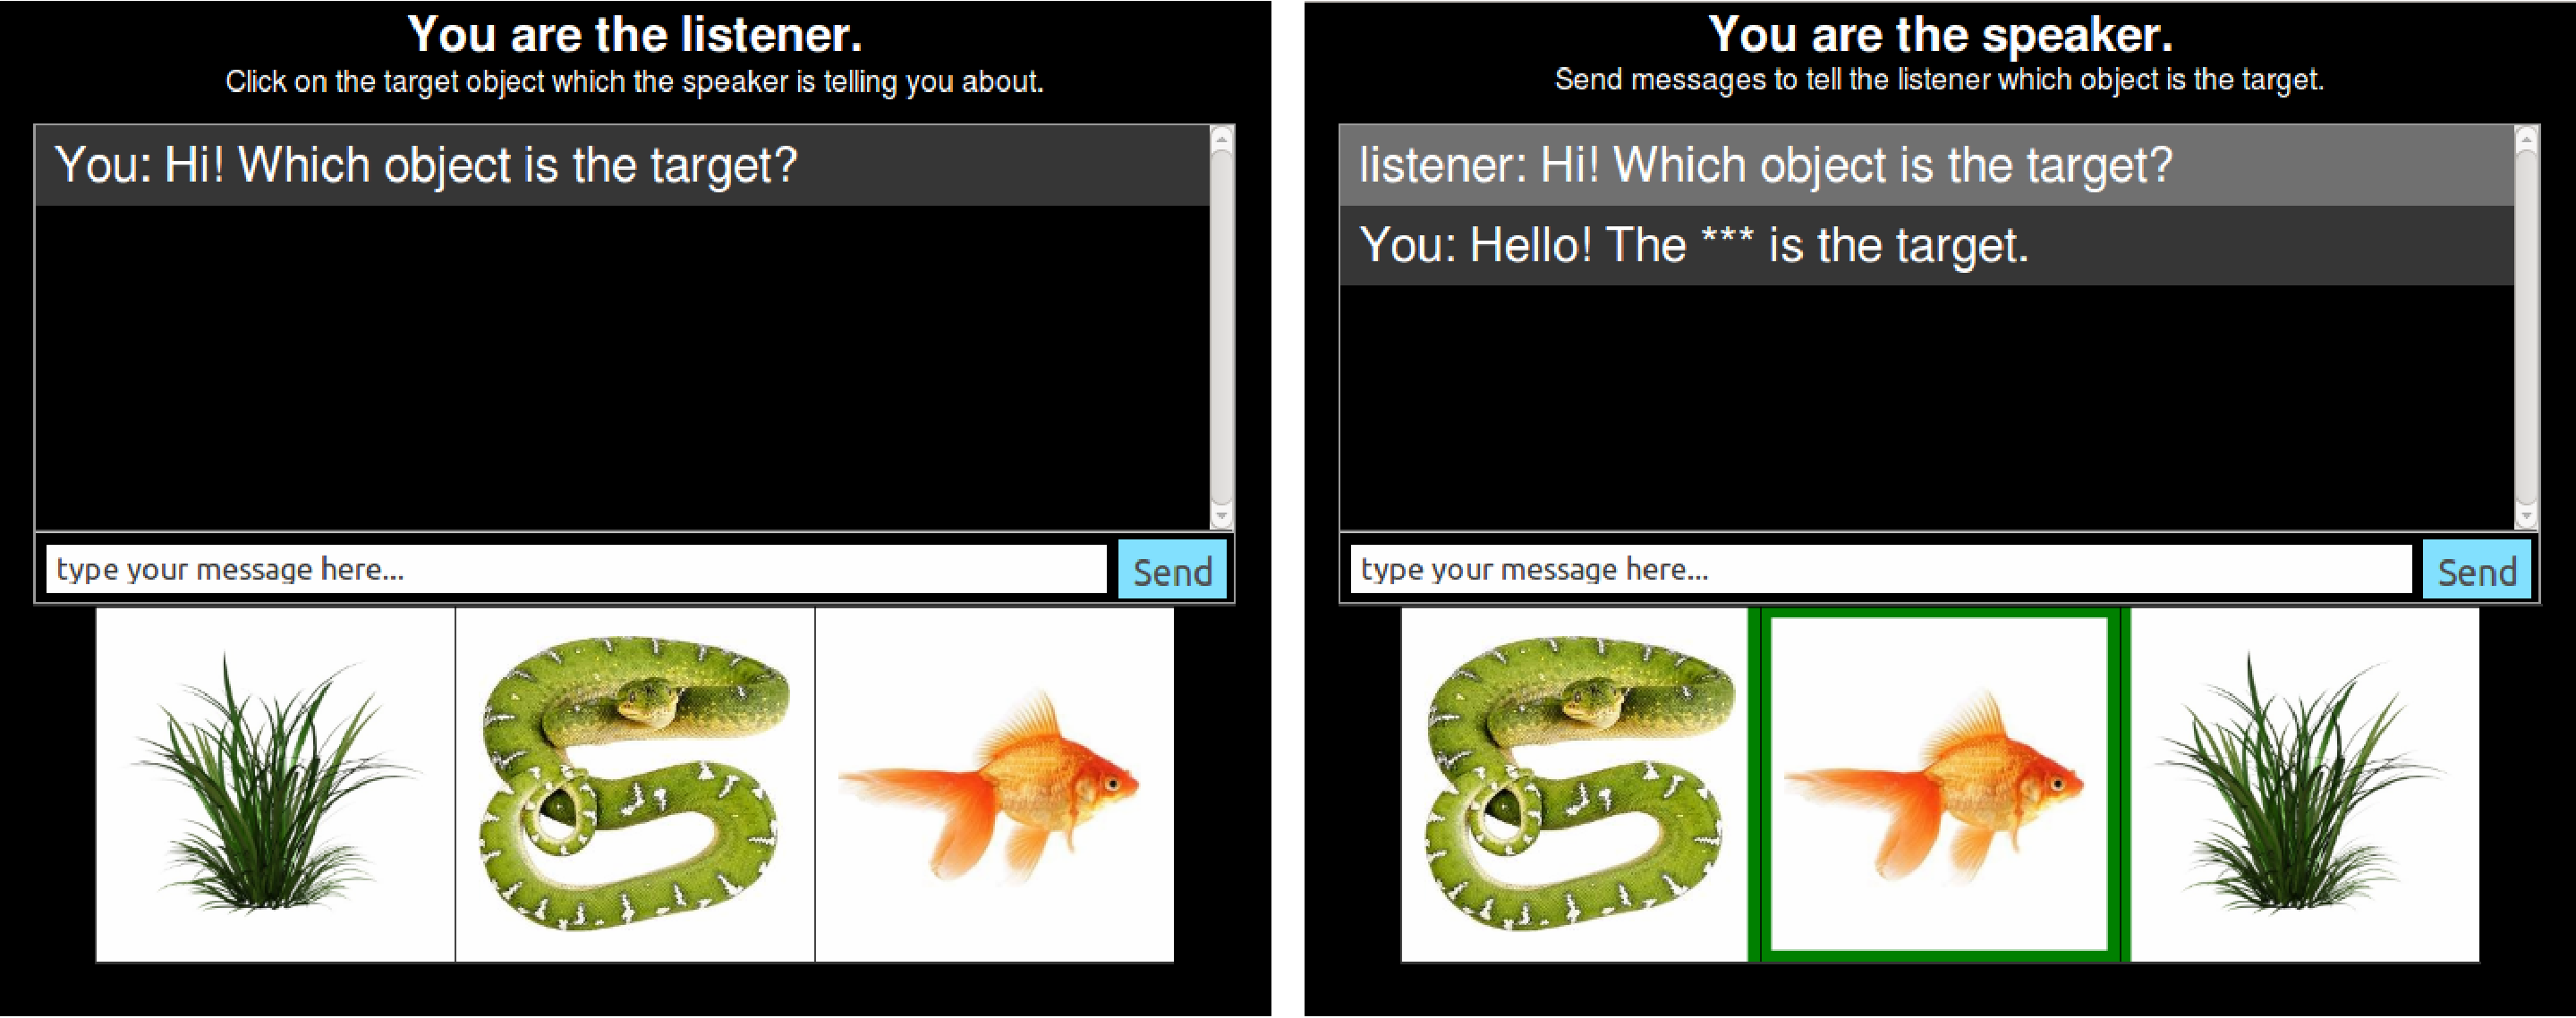
\includegraphics[width=.5\textwidth]{graphs/procedure}
\caption{Screenshots from speakers' and listeners' points of view, showing role names and short task descriptions, the chatbox used for communication and a display of three pictures of objects. The referrent was identified to the speaker by a green box.}
\label{fig:procedure}
\end{figure}

%the choice of level of reference depends on a rich interplay between at least the factors discussed in the previous paragraphs: the contextual informativeness of referring at that level, the utterance's cost (in terms of length and frequency), and the typicality of the referent's properties. What is unknown is how these different factors trade off, and indeed, how a speaker who tries to maximize the communicative efficiency of their utterances, \emph{should} trade off these different factors. 

A promising modeling approach for capturing the quantitative details of human language use is the Rational Speech-Acts (RSA) framework \cite{frank2012, goodmanstuhlmueller2013}.
The RSA framework has been applied to many language interpretation tasks \cite<e.g.>{goodmanstuhlmueller2013,kao2014}, but relatively rarely to production data \cite<but see>{franke2014, Orita2015}. 
We describe an RSA model of nominal reference that includes informativeness, cost, and typicality effects.
A speaker in RSA is treated as an approximately optimal decision maker who chooses which utterance to use to communicate to a listener.
The speaker has a utility which includes terms for the cost of producing an utterance (in terms of length or frequency) and the informativeness of the utterance for a listener.
The listener is treated as a literal Bayesian interpreter who updates her beliefs given the truth of the utterance.
These truth values are usually treated as deterministic (an object either is a ``dog'' or it is not); here we relax this formulation in order to incorporate typicality effects. 
That is, we elicit typicality ratings in a separate experiment, and model the listener as updating her beliefs by weighting the possible referents according to how typical each is for the description used.
We evaluate the quantitative model predictions against our production data.
The model also allows us evaluate the need for each extra component---typicality, length, frequency---and determine whether the empirical bias toward reference at the basic level \cite{RoschEtAl76_BasicLevel} can be accounted for without building it in as a separate factor.

%
%\ndg{put somewhere}
%Moreover, previous research examining the choice of level of reference in nominal expressions found there exists a privileged level of abstraction called the \emph{basic-level} towards which speakers tend to gravitate in free-response naming tasks \cite{RoschEtAl76_BasicLevel}. We aimed to find out to what extent this bias can be accounted for by the three above mentioned factors---contextual informativeness, utterance cost, and typicality. 



\section{Experiment: nominal reference game}

%This experiment investigates the effect of informativeness,  cost, and typicality on the choice of nominal referring expression by varying the visual context of a target object. 
%In our reference game, the participants' visual context consists of a set of two distractor objects. We vary the category level of the distractor objects (same basic level as the target, same superordinate level, different superordinate level) as well as the cost of the subordinate level term compared to the basic level term.
%In order to analyze the effect of cost we collect corpus frequencies and length data from participants' utterances; to incorporate typicality we norm the items with a separate group of participants. 


% We take both an utterance's  length and its frequency to contribute to its overall cost. We also include the typicality norms collected in the previous experiment as predictors of utterance choice.

\subsection{Methods}

%\ndg{i think we want procedure and design figure(s). the procedure fig should show a screen shot from speaker and listener points of view. the design fig should illustrate the dist12, etc notation used later with a concrete domain.}

\paragraph{Participants and materials}
We recruited 56 self-reported native speakers of English over Mechanical Turk. Participants completed the experiment in pairs of two, yielding 28 speaker-listener pairs.

%\paragraph{\bf Materials}
Stimuli were selected from nine distinct domains, each corresponding to distinct basic level categories such as ``dog.'' For each domain, we selected four subcategories to form our target set (e.g. ``dalmatian'', ``pug'', ``German Shepherd'' and ``husky''). Each domain also contained an additional item which belonged to the same basic level category as the target (e.g. ``greyhound'') and items which belonged to the same supercategory but not the same basic level (e.g. ``elephant'' or ``squirrel''). The latter items were used as distractors.

%\paragraph{\bf Design}
Each trial consisted of a display of three images, one of which was designated as the target object. Every pair of participants saw every target exactly once, for a total of 36 trials per pair. These target items were randomly assigned distractor items which were selected from four different context conditions, corresponding to different communicative pressures (see Fig. \ref{fig:design}). We refer to these conditions with pairs of numerals specifying which levels of the taxonomy are present in the distractors: (a) \textbf{item12}: one distractor of the same basic level and one distractor of the same superlevel (e.g. target: ``dalmatian'', distractor 1: ``greyhound'', distractor 2: ``squirrel''), (b) \textbf{item22}: two distractors of the same superlevel, (c) \textbf{item23}: one distractor of the same superlevel and one unrelated item and (d) \textbf{item33}: two unrelated items.

% \todo[inline]{rdh: would be nice to use the TeX \emph{description} environment to format this if we have room} Each pair saw nine trials in each condition. 
%\todo[inline]{rdh: maybe it should already be clear from this, but how did we assign contexts to the 36 items? Totally randomly (with this 9 trials/condition constraint)? Or did the four targets within a domain get a one-to-one mapping with the four conditions?} (caroline: Yes it was totally random, except for 9 trials/condition constraint and every one of the 36 targets used once.)

Furthermore, the experiment contained 36 filler items, in which participants were asked to produce referential expressions for objects which differed only in size and color. Images from filler trials were not reused on target trials. Trial order was randomized. 

\begin{figure}[bt!]
\centering
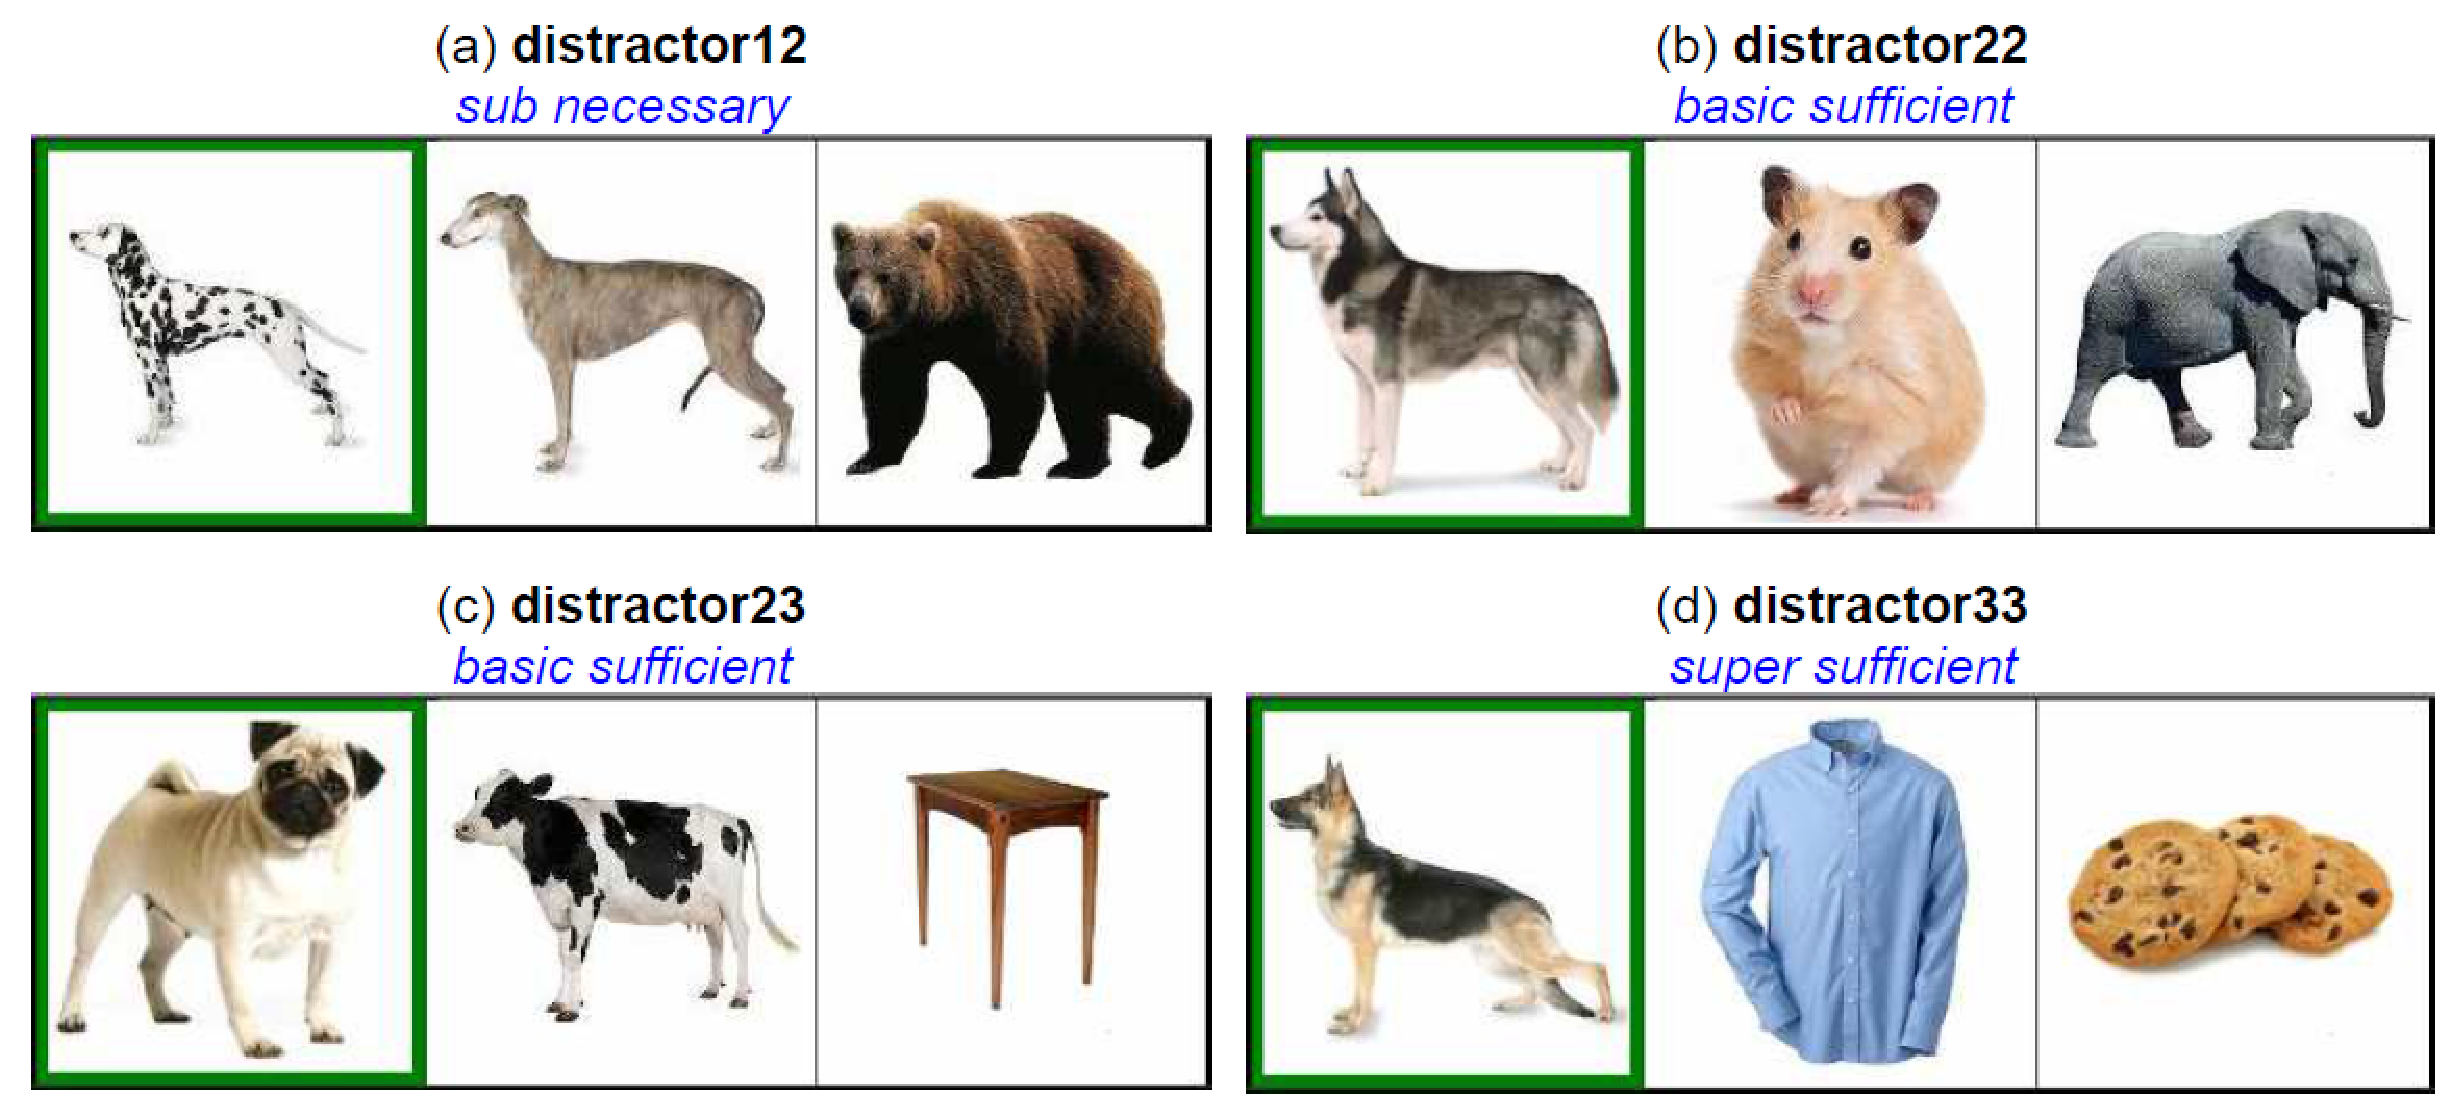
\includegraphics[width=.5\textwidth]{graphs/design}
\caption{The four context conditions, exemplified by the \textit{dog} domain. The target is outlined in green; the types of distractors differ with condition (see text).
%: in the  \textbf{item12} condition, a distractor of the same basic level as the target (i.e. a distractor class 1) and a distractor of the same super level as the target (i.e. a distractor class 2) is presented. In \textbf{item22}, both distractors are class 2 distractors. In \textbf{item23}, one distractor is a class 2 distractor and the other is an artifact which neither shares the basic level nor super level with the target (i.e. a distractor class 3). Finally, there are two class 3 distractors in \textbf{item33}.
%\ndg{we call these item12 etc elsewhere. should adjust.}
}
\label{fig:design}
\end{figure}

\paragraph{Procedure}
Pairs of participants were connected through a real-time multi-player interface \cite{Hawkins15_RealTimeWebExperiments}, with one member of each pair assigned the speaker role and the other to the listener role. Participants kept their allotted roles for the entire experiment. 
The setup for both the speaker and the listener is shown in \figref{fig:procedure}. Each saw the same set of three images, but positions were randomized to rule out trivial position-based references like ``the middle one.'' The target object was identified by a green square surrounding it for the speaker (but not listener). Players used a chatbox to send text messages to each other. The task was for the speaker to get the listener to select the target object. %, and for the listener to select the right object based on the information provided by the speaker. 

\paragraph{Annotation}
To determine the level of reference for each trial, we followed the following procedure. First, trials on which the listener selected the wrong referent were excluded, leading to the elimination of 1.2\% of trials. Then, speakers' and listeners' messages were parsed automatically; the referential expression used by the speaker was extracted for each trial and checked for whether it contained the current target's correct sub, basic or super level term using a simple grep search. In this way, 66.2\% of trials were labelled as mentioning a pre-coded level of reference. In the next step, remaining utterances were checked manually to determine whether they contained a correct level of reference term which was not detected by the parsing algorithm due to typos or grammatical modification of the expression. In this way, meaning-equivalent alternatives such as ``doggie'' for ``dog'',  or contractions such as ``gummi'',``gummies'' and ``bears'' for ``gummy bears'' were counted as containing a level of reference term. This caught another 13.8\% of trials. A total of 20.0\% of correct trials were excluded because the utterance consisted only of an \emph{attribute} of the superclass (``the living thing'' for ``animal''), of the basic level (``can fly'' for ``bird''), of the subcategory (``barks'' for ``dog'') or of the  particular instance (``the thing facing left'') rather than a category noun. These kinds of attributes were also sometimes mentioned in addition to the noun in the trials which were included in the analysis---4.0\% of sub level terms, 12.6\% of basic level terms, and 46.2\% of super level terms contained an additional modifier. 
%By making use of attributes,  speakers could generate unambiguous referential expressions despite using a level of reference which would by itself be insufficient for disambiguation, e.g. by referring to a dalmatian as a ``spotted dog'' (in the context of another dog being present, for instance a pug which is not spotted). 
On 0.5\% of trials two different levels of reference were mentioned; in this case the more specific level of reference was counted as being mentioned in this trial. 
%Additional processing also established the number of correct trials where a determiner (``the'' or ``a''/``an'') or an indefinite referent such as ``one'', ``thing'' or ``object'' was used, how many correct trials consisted of complete sentences and the number of correct trials where level of reference terms were contracted (namely 2.7\%, 0.9\%, 1.0\% and 5.3\% respectively). \jd{do we need the last bit of info, since we don't actually go on to do anything with it?}

%\todo[inline]{rdh: i don't think these numbers  add up to 100... 1.2 were incorrect and excluded, (66.2 + 13.8) were correct and included, 10\% of the total correct ones were excluded $= 91.2$ at most. Or maybe I'm counting wrong, in which case we should maybe find a less confusing way of expressing these probabilities?} \caroline{Sorry! very embarassing typo. Of all trials, 1.2\% were incorrect and thus excluded. Of the remaining *correct* trials, 66.2\% were labelled in the first automatic parse, then another 13.8\% were added manually, so 80.0\% of correct trials were labelled as mentioning a level of reference. The remaining 20.0\% of correct trials mentioned an attribute and were thus excluded (not 10.0\%!!) (resolved)}

\paragraph{Typicality norms}

To examine the influence of typicality on speaker behavior, we obtained typicality estimates in a separate norming study. 240 participants were recruited through Mechanical Turk. On each trial, we presented participants with an image from the main experiment and asked them ``How typical is this for X?'', where X was a category label at the sub-, basic-, or super- level. They then adjusted a slider bar ranging from \emph{not at all typical} to \emph{very typical}. 

Due to the large number of possible combinations of objects, we only collected norms for certain combinations of objects and descriptions: for each target (e.g., dalmatian), we collected typicality at all three levels (``dalmatian,'' ``dog,'' and ``animal''). For each distractor of the same superclass as the target (\emph{distsamesuper}, e.g., a kitten), we collected typicality at all three levels of the \emph{target}. For each distractor of a different superclass (\emph{distdiffsuper}, e.g., a basketball) we only collected typicality at the super- level of the target (``animal'') and assumed lowest typicality at the other levels. This resulted in the following distribution of 745 norms:  \emph{target-sub} (36), \emph{target-basic} (36), \emph{target-super} (36), \emph{distdiffsuper-super} (168), \emph{distsamesuper-sub} (331), \emph{distsamesuper-basic} (93), and \emph{distsamesuper-super} (45). 

Each participant provided typicality ratings for 7 \emph{target}, 10 \emph{distdiffsuper}, and 28 \emph{distsamesuper} cases (randomly sampled from the total set of items). Each case received between 6 and 27 ratings.  Raw slider values ranged from 0 (not typical) to 1 (very typical); average slider values were used as the typicality values throughout our results. 

\subsection{\bf Results}

Proportions of sub, basic, and super level utterance choices in the different context conditions are shown in the top row of \figref{fig:qualitativemodel}. The sub level term was preferred where it was necessary for unambiguous referent identification, i.e., when a distractor of the same basic level category as the target was present in the scene (item12, e.g. target: dalmatian, distractor: greyhound). Where it was not necessary (i.e., when there was no other object of the same basic level category present, as in conditions item22, item23 and item33), there was a clear preference for the basic level term. The super level term was strongly dispreferred overall, though it was used on some trials, especially where informativeness constraints on utterance choice were weakest (item33). 
%
%\begin{figure}[ht!]
%\centering
%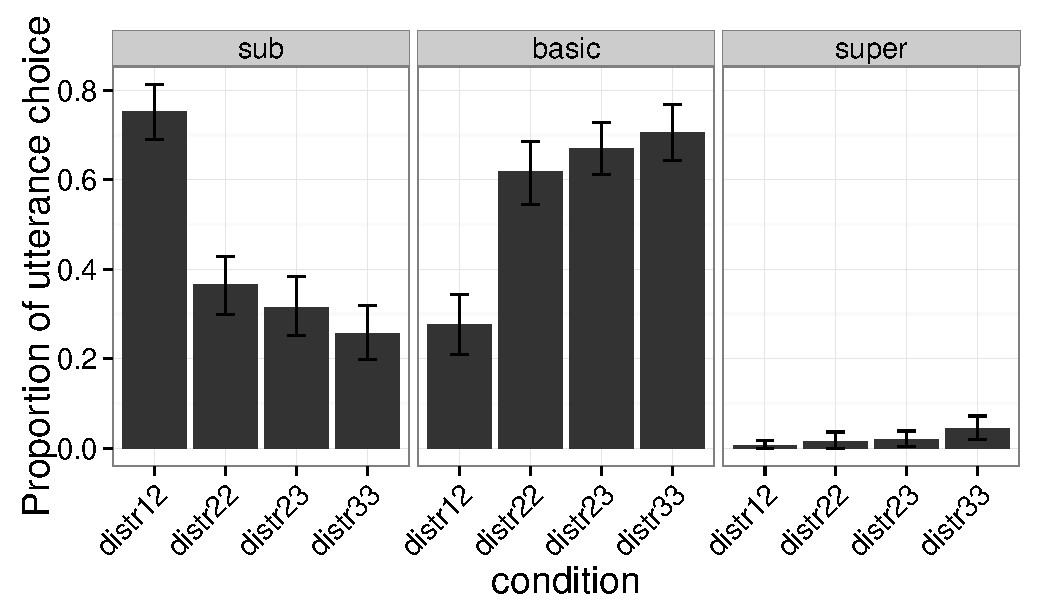
\includegraphics[width=.5\textwidth]{graphs/results-collapsed}
%\caption{Proportion of utterance choice by condition. Error bars indicate bootstrapped 95\% confidence intervals.}
%\label{fig:results1}
%\end{figure}

To test for the independent effects of informativeness, length, frequency, and typicality on sub-level mention, we conducted a mixed effects logistic regression. Frequency was coded as the difference between the sub and the basic level's log frequency, as extracted from the Google Books Ngram English corpus ranging from 1960 to 2008. Length was coded as the ratio of the sub to the basic level's length.\footnote{We used the mean empirical lengths in characters of the utterances participants produced. For example, the minivan, when referred to at the subcategory level, was sometimes called ``minivan'' and sometimes ``van'' leading to a mean empirical length of 5.64. This is the value that was used, rather than 7, the length of ``minivan''.} That is, a higher frequency difference indicates a \emph{lower} cost for the sub level term compared to the basic level, while a higher length ratio reflects a \emph{higher} cost for the sub level term compared to the basic level. Typicality was coded as the ratio of the target's sub to basic level label typicality. That is, the higher the ratio, the more typical the object was for the sub level label compared to the basic level.
%; or in other words, a higher ratio indicated that the object was relatively atypical for the basic label compared to the sub label. 
For instance, the panda was relatively atypical for its basic level ``bear'' (mean rating 0.75) compared to the sub level term ``panda bear'' (mean rating 0.98), which resulted in a relatively \emph{high} typicality ratio.

\begin{figure}[bt]
\centering
%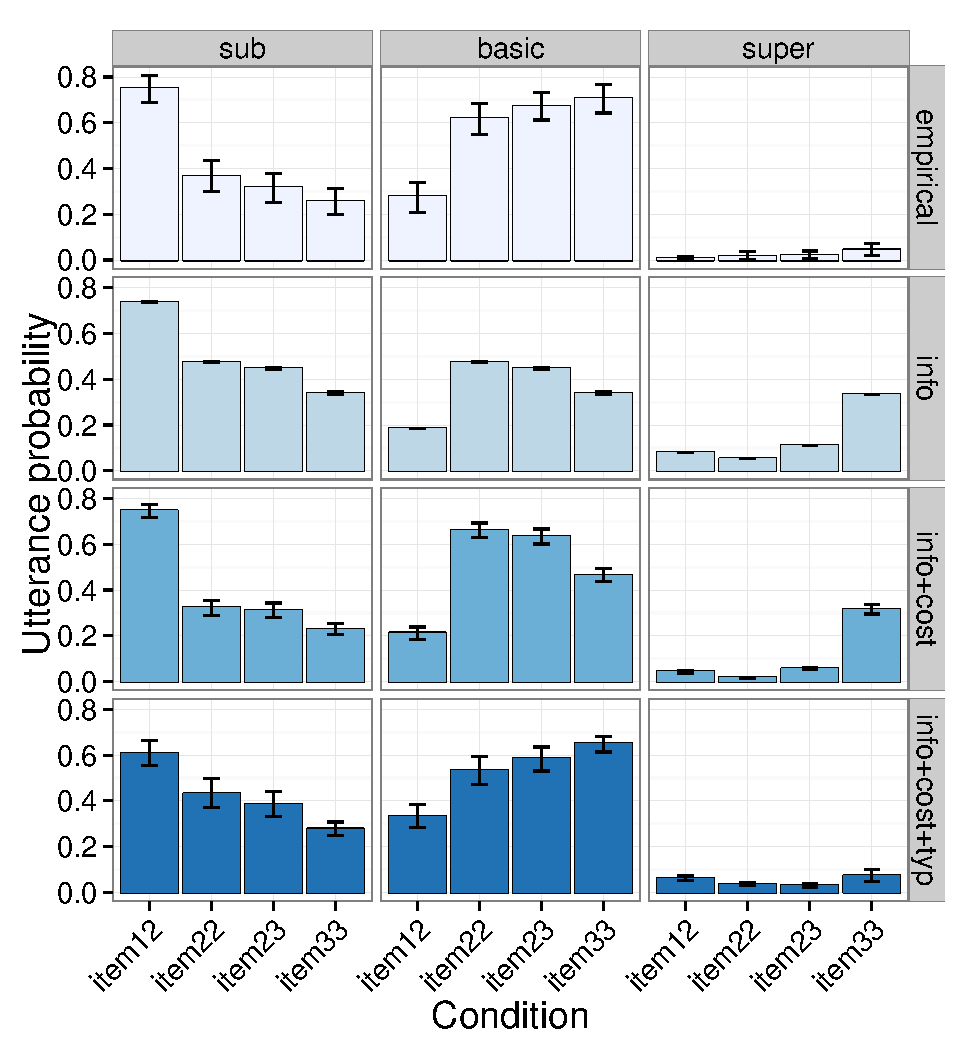
\includegraphics[width=.5\textwidth]{graphs/collapsed-pattern}
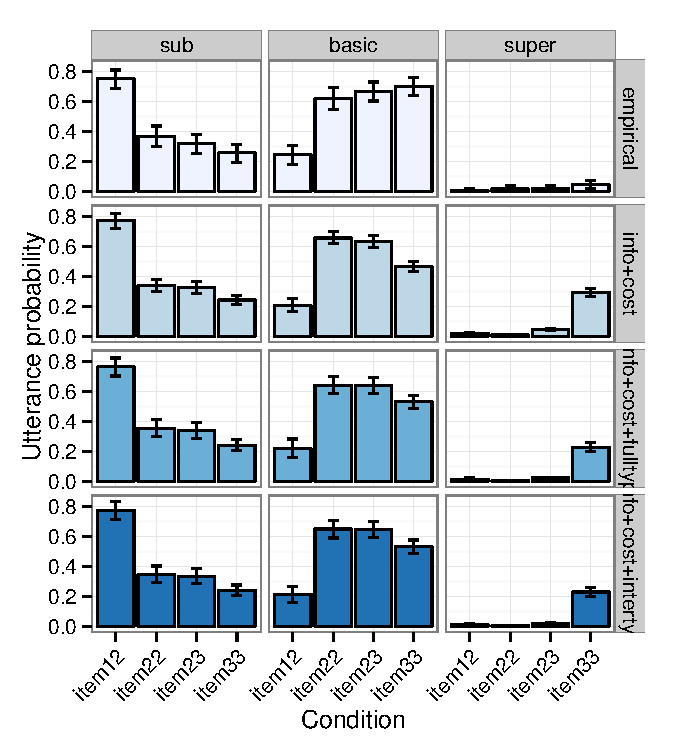
\includegraphics[width=.5\textwidth]{graphs/qualitativepattern}
\caption{Empirical utterance probabilities (top row) and model posterior predictive means (bottom row) by condition, collapsed across targets and domains. Error bars indicate bootstrapped 95\% confidence intervals.}
\label{fig:qualitativemodel}
\end{figure}

Condition was coded as a three-level factor: \emph{sub necessary}, \emph{basic sufficient}, and \emph{super sufficient}, where item22 and item23 were collapsed into \emph{basic sufficient}. Condition was Helmert-coded: two contrasts over the three condition levels were included in the model, comparing each level against the mean of the remaining levels (in order: \emph{sub necessary}, \emph{basic sufficient}, \emph{super sufficient}). This allowed us to determine whether the probability of type mention  for neighboring conditions were significantly different from each other, as suggested by \figref{fig:qualitativemodel}.\footnote{Adding terms that code the ratio of the sub vs super level frequency and length did not lead to an improvement of model fit.} The model included random by-speaker and by-domain intercepts. 

A summary of results is shown in \tableref{tab:modelresults}. The log odds of mentioning the sub level term was greater in the \emph{sub necessary} condition than in either of the other two conditions, and greater in the \emph{basic sufficient} condition than in the \emph{super sufficient} condition, suggesting that the contextual informativeness of the sub level mention has a gradient effect on utterance choice. There was also a main effect of typicality, such that the sub level term was preferred for objects that were more typical for the sub level compared to the basic level  description (see \figref{fig:lengthtypicality}). In addition, there was a main effect of length, such that as the length of the sub level term increased compared to the basic level term (``chihuahua''/``dog'' vs.~``pug''/``dog''), the sub level term was dispreferred (i.e., ``chihuahua'' is dispreferred compared to ``pug'', see \figref{fig:lengthtypicality}). Finally, while there was no main effect of frequency, we observed a significant length by frequency interaction, such that there was a frequency effect for the relatively shorter but not the relatively longer sub level cases: for shorter sub level terms, relatively high-frequency sub level terms were more likely to be used than relatively low-frequency sub level terms. 

\begin{table}[tbp]
\caption{Mixed effects model summary.}
\begin{center}
\begin{tabular}{lrrl}
\toprule
\multicolumn{1}{l}{}&\multicolumn{1}{c}{Coef $\beta$}&\multicolumn{1}{c}{SE($\beta$)}&\multicolumn{1}{c}{$p$}\tabularnewline
\midrule
Intercept&$-0.30$&$0.35$&\textgreater0.4\tabularnewline
Condition sub.vs.rest&$ 2.46$&$0.24$&\textbf{\textless.0001}\tabularnewline
Condition basic.vs.super&$ 0.52$&$0.23$&\textbf{\textless.05}\tabularnewline
Length&$-0.52$&$0.14$&\textbf{\textless.001}\tabularnewline
Frequency&$-0.02$&$0.08$&\textgreater0.78\tabularnewline
Typicality&$ 4.17$&$0.84$&\textbf{\textless.0001}\tabularnewline
Length:Frequency&$-0.30$&$0.11$&\textbf{\textless.01}\tabularnewline
\bottomrule
\end{tabular}\end{center}
\label{tab:modelresults}
\end{table}



%\begin{figure}[ht!]
%\centering
%%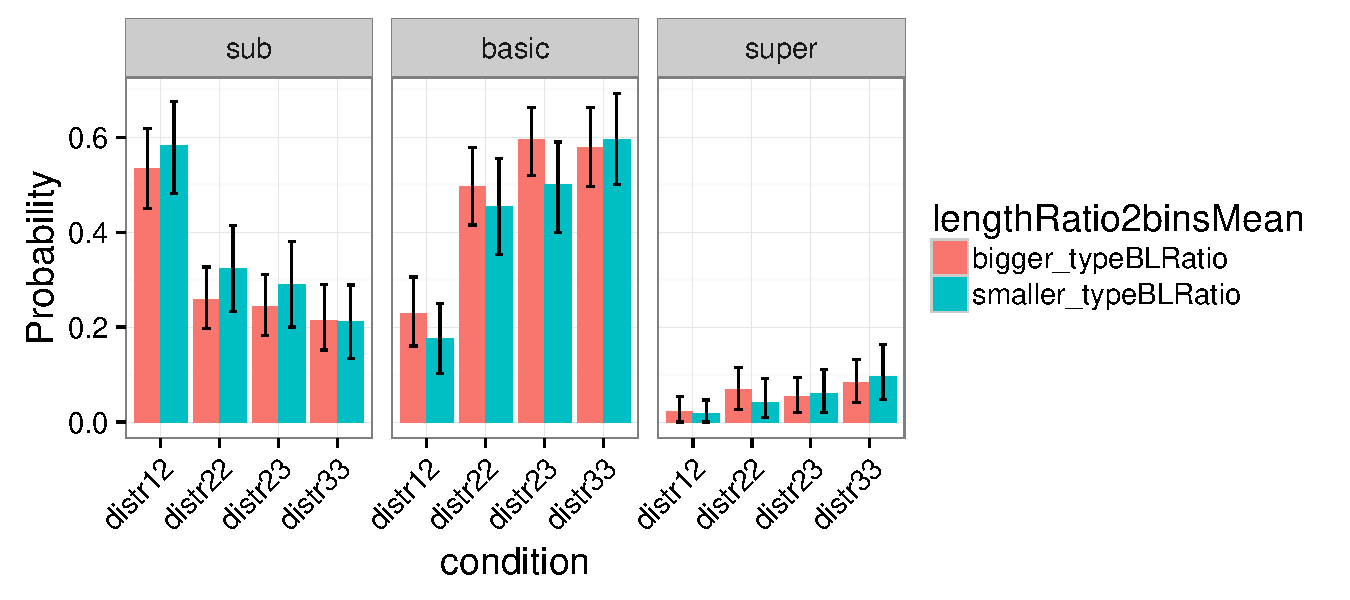
\includegraphics[width=.5\textwidth]{graphs/lengthRatio}
%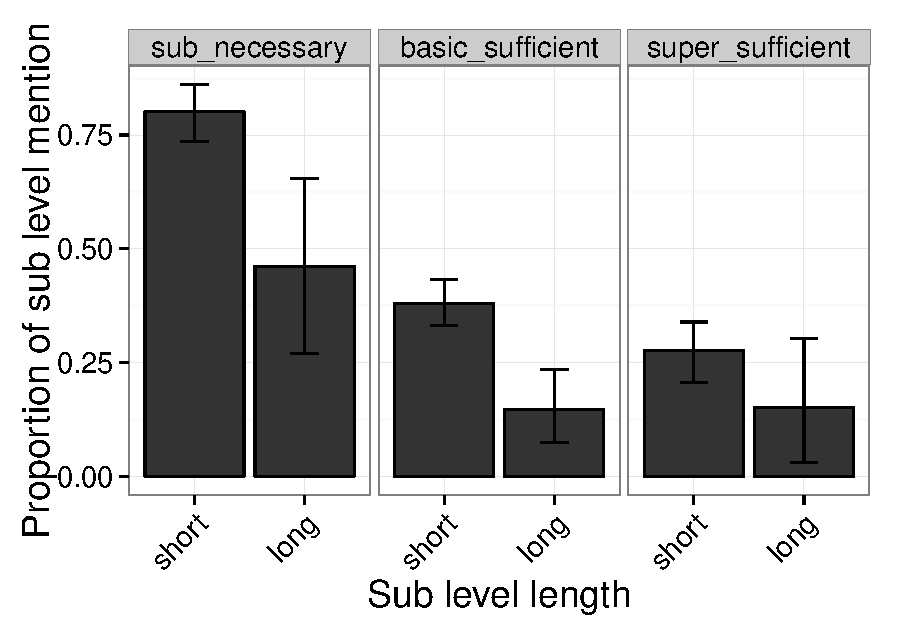
\includegraphics[width=.5\textwidth]{graphs/length-effect}
%\caption{Probability of using sub, basic and super level terms when the sub  length is relatively short (.67,2] or long [2,4.67) compared to the basic level term length.}
% \label{fig:lengtheffect}
%\end{figure}


%
%\begin{figure}[ht!]
%\centering
%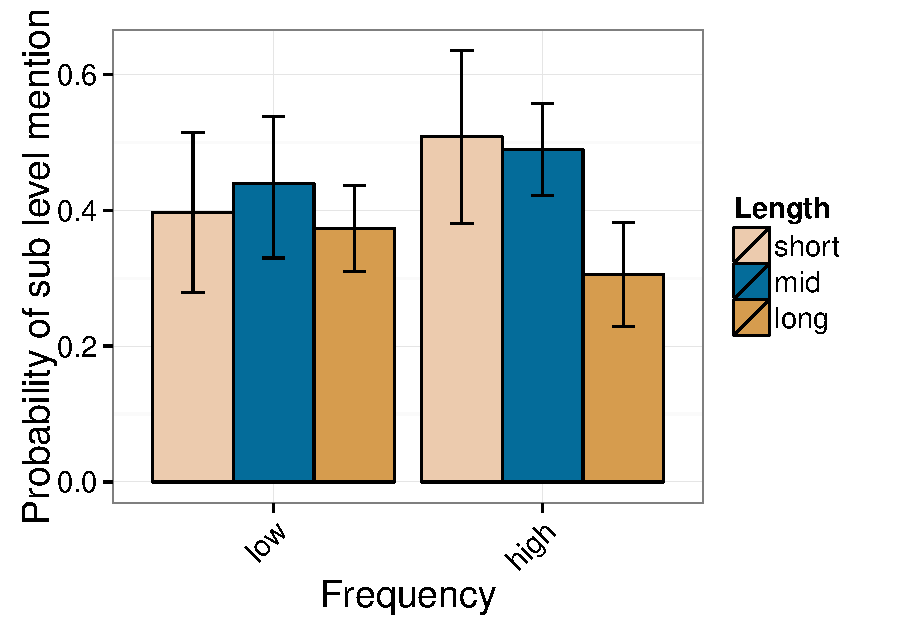
\includegraphics[width=.5\textwidth]{graphs/freq-length-interaction}
%\caption{Proportion of sub level mentions  as a function of the sub level term's relative length and frequency compared to the basic level. Length bins reflect the sub/basic length ratio intervals (0, 1] (short), (1, 2] (mid), (2, 4.67] (long). Frequency bins reflect the sub/basic log frequency difference intervals (-11.2,-5.19] (low), (-5.19,-0.65] (high).}
%\label{fig:lengthfreqinteraction}
%\end{figure}


Unsurprisingly, there was also significant by-participant and by-domain variation in the log odds of sub level term mention. %\figref{fig:bigscatterplot} shows the by-domain variation in utterance choice. 
For instance, mentioning the subclass over the basic level term was preferred more in some domains (e.g. in the ``candy'' domain) than in others. Likewise, some domains had a greater preference for basic level terms (e.g. the ``shirt'' domain). Using the superclass term also ranged from hardly being observable (e.g. the ``flower'' domain) to being used more frequently (e.g. in the ``bird'' domain). Nevertheless, mentioning the sub level term was always the most frequent choice where a distractor of the same basic level was displayed. Furthermore, it was the case in all domains that the sub level term was mentioned most frequently and the basic level least frequently in just this condition, compared to the other three conditions.


%These results suggest that the choice of level of reference depends in a gradient manner on both the informativeness of the reference level as well as on the fit of the object to a specific label due to typicality and the cost of the corresponding utterance (in terms of length combined with frequency) compared to the alternative utterances. [caroline: I moved this to the conclusion section]


\begin{figure}[bt]
\centering
%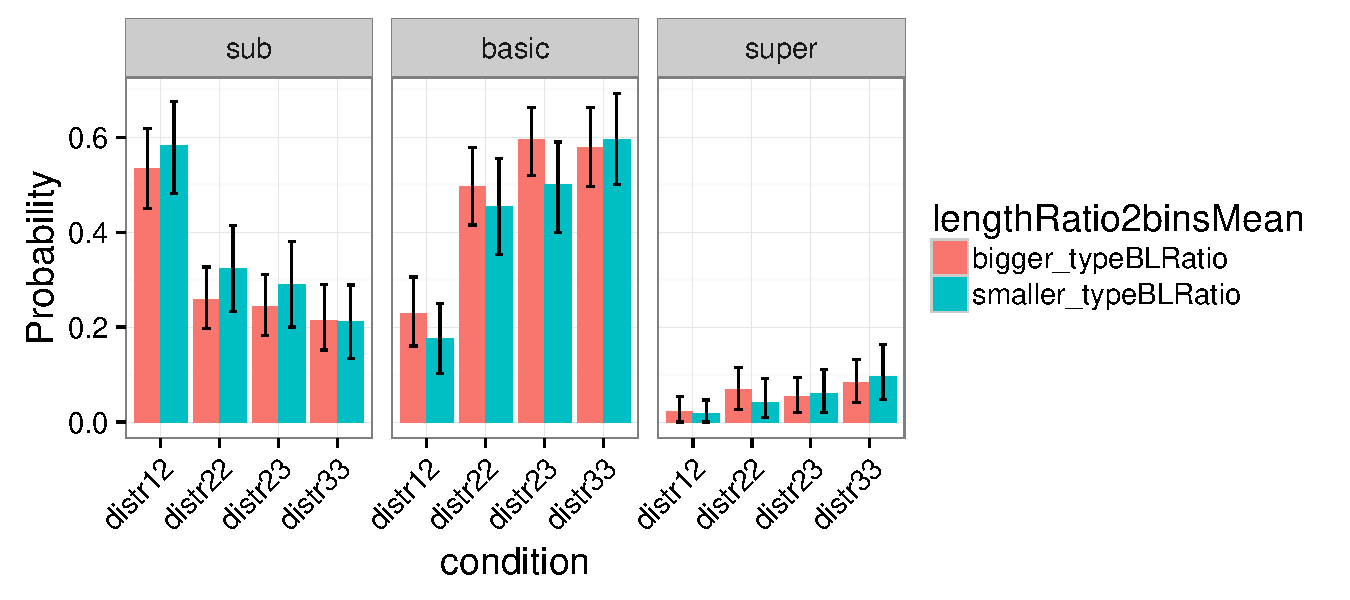
\includegraphics[width=.5\textwidth]{graphs/lengthRatio}
%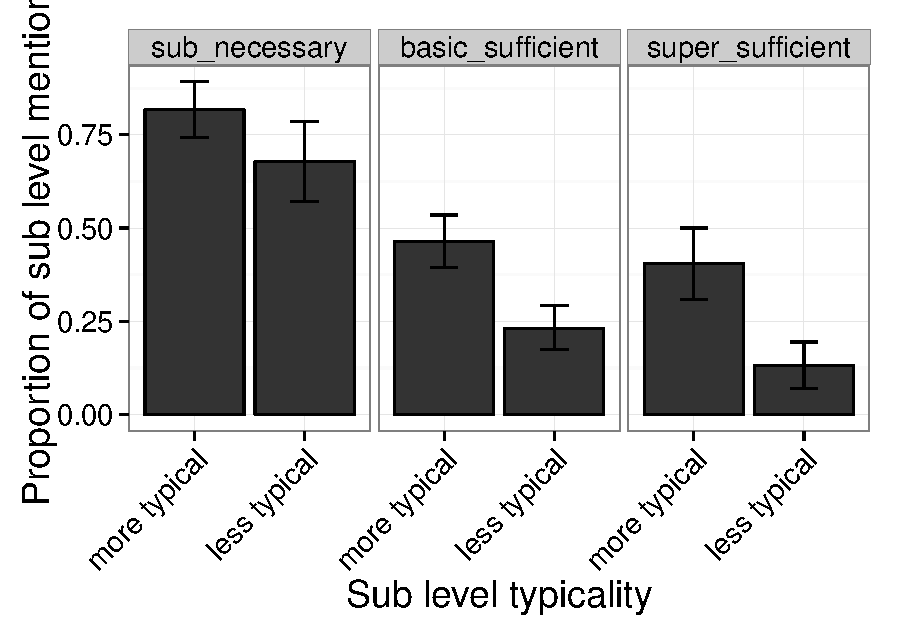
\includegraphics[width=.5\textwidth]{graphs/typicality-effect}
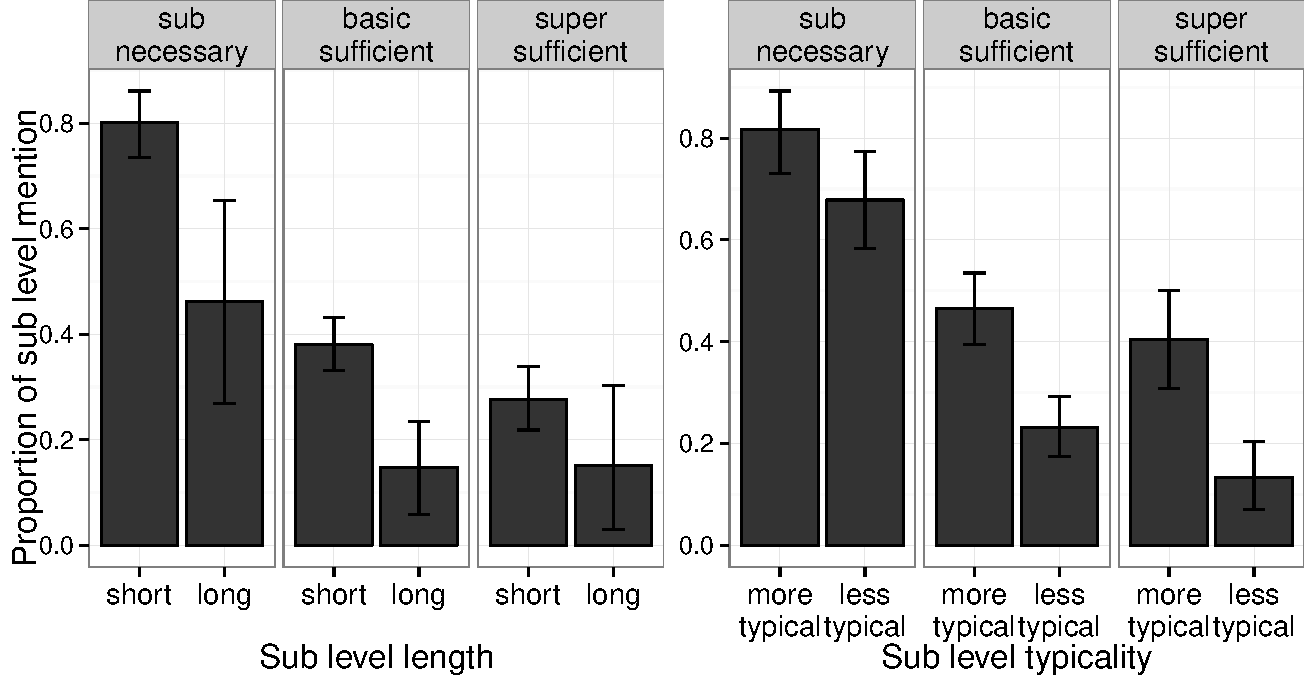
\includegraphics[width=.5\textwidth]{graphs/length-typicality}
\caption{Probability of using sub, basic and super level terms. Left: when the sub  length is relatively short (.67,2] or long [2,4.67) compared to the basic level term length. Right: when the target object was relatively more [1.06,1.91) or less (.88,1.06] typical for the sub compared to the basic level term.}
 \label{fig:lengthtypicality}
\end{figure}


\section{\bf Modeling level of reference}

%To show that we can account for these context effects purely through communicative pressures, we formulated a simple probabilistic model of basic level reference. 
We formulated a probabilistic model of reference level selection that integrates contextual informativeness, utterance cost, and typicality.
As in earlier Rational Speech-Acts (RSA) models \cite{frank2012, goodmanstuhlmueller2013}, the speaker seeks to be informative with respect to an internal model of a literal listener. This listener updates her beliefs to rule out possible worlds that are inconsistent with the meaning of the speaker's utterance. Rather than assuming that words have deterministic truth conditions, as has usually been done in the past, we account for typicality by allowing each label a graded meaning. For instance, the word ``dog'' describes a dalmatian better than a grizzly bear, but it also describes a grizzly bear better than a tennis ball.
The speaker also seeks to be parsimonious: the speaker utility includes both informativeness and word cost; cost includes both length and frequency.

Formally, we start by specifying a literal listener $L_0$ who hears a word $l$ at a particular level of reference  in the context of some set of objects $\mathcal{O}$ and forms a distribution over the referenced object, $o \in \mathcal{O}$ : 
$$P_{L_0}(o | l) \propto \denote{l}(o).$$
Here $\denote{l}(o)$ is the lexical meaning of the word $l$ when applied to object $o$. We take this to be a real number indicating the degree of acceptability of object $o$ for category $l$. 
We relate this to our empirically elicited typicality norms via an exponential relationship: $\denote{l}(o)=\exp(\text{typicality}(o,l))$.\footnote{Cases where typicality was not elicited were assumed to have typicality $0$.}
This relationship is motivated by considering the effect of a small difference in typicality on choice probability: in our elicitation experiment a small difference in rating should mean the same thing at the top and bottom of the scale (it is visually equivalent on the slider that participants used).
In order for a small difference in typicality rating to have a constant effect on relative choice probability (which is a ratio), the relationship must be exponential. 
%The parameter $\gamma$ controls the dynamic range of typicality---how good (bad) is it to choose an object which is very (a)typical of the label heard?

Next, we specify a speaker $S_1$ who intends to refer to a particular object $o \in \mathcal{O}$ and chooses among possible nouns $l \in {\mathcal L}(o)$.
We take ${\mathcal L}(o)$ to be the three labels for $o$ at sub, basic, and super level.
The speaker chooses among these nouns in a way that is influenced by informativeness of the noun for the literal listener ($\ln P_{L_0}(o | l)$), the frequency ($\hat{c}_f$) and the length  ($\hat{c}_l$), each weighted by a free parameter:
$$P_{S_1}(l | o) \propto \exp(\lambda \ln P_{L_0}(o | l) + \beta_f \hat{c}_f  + \beta_l \hat{c}_l)$$
Length cost $\hat{c}_l$ was defined as the empirical mean number of characters used to refer at that level and frequency cost $\hat{c}_f$ was the log frequency in the Google Books corpus from 1960 to the present. 

We performed Bayesian data analysis to generate model predictions, conditioning on the observed production data (coded into sub, basic, and super labels as described above) and integrating over the three free parameters.
We assumed uniform priors for each parameter: $\lambda  \sim Unif(0,20)$, $\beta_f \sim Unif(0,5)$, $\beta_l \sim Unif(0,5)$.
We implemented both the cognitive and data-analysis models in the probabilistic programming language WebPPL \cite{GoodmanStuhlmuller14_DIPPL}.
Inference for the cognitive model was exact, while we used Markov Chain Monte Carlo (MCMC) to infer posteriors for the three free parameters.
% using Markov Chain Monte Carlo (MCMC), conditioning on the production data from the experiment reported above. More specifically, for every iteration of the chain, we generated the probability of a speaker using each level of reference (i.e .``sub'', ``basic'', or ``super'') for every \emph{context} that participants could encounter in the task, and then computed the likelihood of the actual expressions that participants used. 

\begin{figure}[t!]
\centering
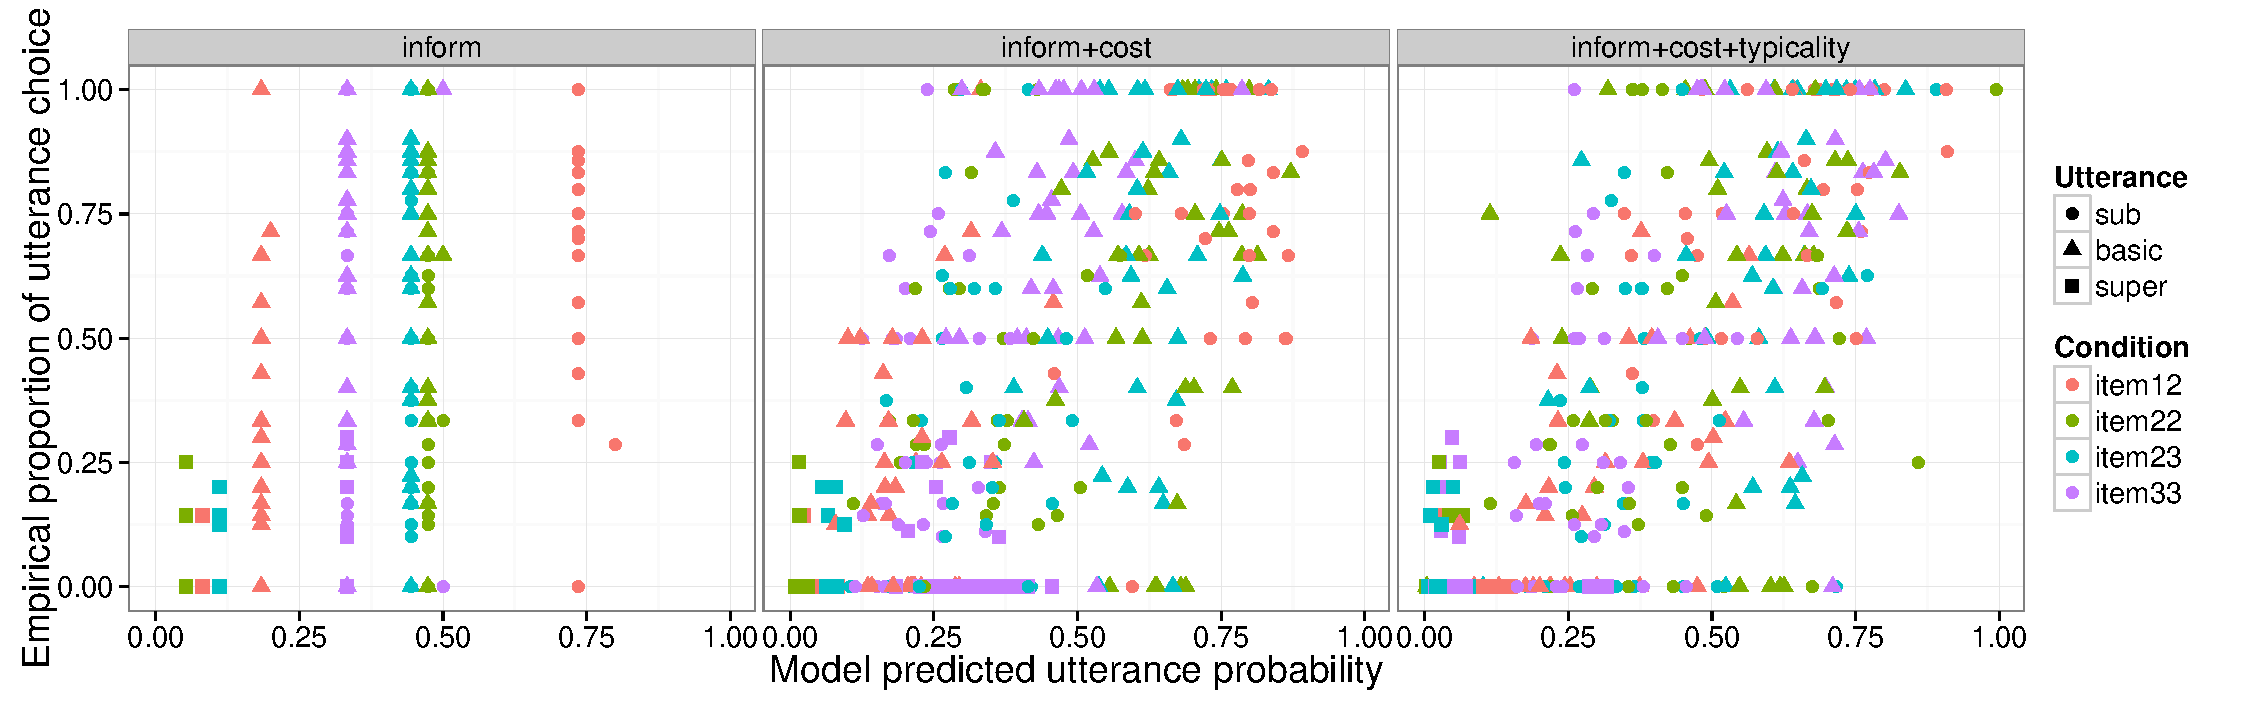
\includegraphics[width=.45\textwidth]{graphs/scatterplot}
\caption{Empirical production data for each level of reference against model posterior predictive at the by-target level.}
 \label{fig:scatterplot}
\end{figure}

Posterior predictions of the model at the target level (collapsing across distractors for each target, within each condition) are compared to empirical data in Fig. \ref{fig:scatterplot}. On the by-target level the model achieves a correlation of $r = .79$. Looking at results on the by-domain level (collapsing across targets) and on the by-condition level (further collapsing across domains, as in \figref{fig:qualitativemodel}) yields correlations of .88 and .96, respectively. 
The model does a good job of capturing the quantitative patterns in the data, especially considering the sparsity of our data at the by-target level.
One clear flaw is that the model predicts greater use of the super level label than people exhibit.
Further systematic deviation appears likely for specific items. 
On examination, candy items like ``gummy bears'' or ``jelly beans'' were particularly problematic, being referred to primarily by their sub level term in all contexts.

\begin{figure}
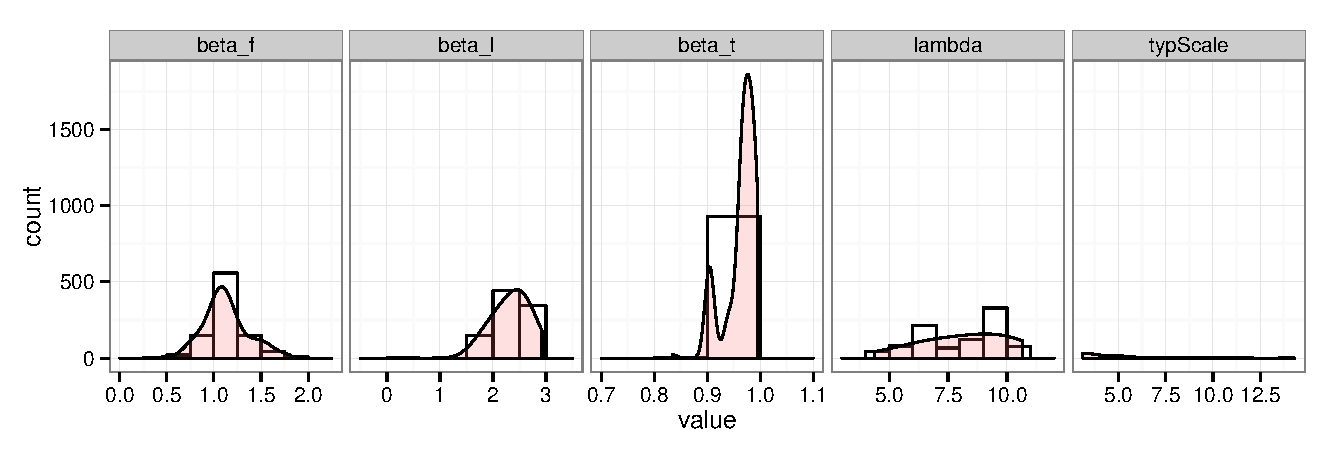
\includegraphics[width=.45\textwidth]{graphs/parameterposteriors.pdf}
\caption{Posterior distribution over model parameters. Maximum a posteriori (MAP) $\lambda = 10.8$, 95\% highest density interval (HDI) $= [9.7, 12.8]$; MAP $\beta_l = 2.5$, HDI $= [1.9, 3.1]$; MAP $\beta_f = 1.3$, HDI $= [0.8, 1.8]$.}
\label{fig:paramposteriors}
\end{figure}

Parameter posteriors are presented in Fig. \ref{fig:paramposteriors}. 
Informativeness is weighted relatively strongly, while length is weighted somewhat more strongly than frequency.
Because this model contains the simpler models without frequency, length, and informativity as nested sub-models, we can use parameter posteriors for Bayesian model selection.
In this case the 95\% highest density intervals (HDIs) exclude zero for each of the three weight parameters, indicating that each term is justified.
In order to ascertain whether typicality was indeed contributing to the explanatory power of the model, we ran an additional Bayesian data analysis with an added typicality weight parameter $\beta_t \in [0,1]$. This parameter interpolated between empirical typicality values (when $\beta_t {=} 1$) and deterministic (i.e. $0$ or $1$) \emph{a priori} values based on the true taxonomy (when $\beta_t {=} 0$).
%truth-conditional function returning one if the object was a member of the label category and zero otherwise. 
%The posterior distribution of this parameter allows for Bayesian model selection: if $\beta_t = 0$ is excluded from the HDI, and the distribution skews high, then some influence of typicality is necessary to account for the data. 
We found a MAP estimate for $\beta_t$ of $.94$, HDI $= [0.88,1]$, strongly indicating that empirical typicality values are necessary.  
Finally, we ran a model including a parameter weighting the \emph{product} of frequency and cost, corresponding to the interaction term in our regression analysis. Its posterior distribution was strongly peaked at 0, indicating that any contribution of the interaction is already captured by other aspects of the model. 
%: one that included only an informativeness term (\tableref{tab:bestparams}, first row and \figref{fig:qualitativemodel}, second row) and one that included informativeness and the cost terms but no typicality (\tableref{tab:bestparams}, second row and \figref{fig:qualitativemodel}, third row). 
%The model without typicality performed significantly worse, as \red{can be seen in the lower correlations of the simpler models .
% Interestingly, as model complexity increases, informativeness is given more weight (as can be seen in the increasing best $\lambda$ value), the extreme effects of which are balanced out by cost and typicality.}




\section{\bf Discussion and conclusion}

%\ndg{things to say: we got naturalistic data of nominal reference. this was affected by cost (length), context, and typicality. these factors fit naturally into an RSA model. this predicts basic level bias without building it in, and interactions between these factors. future work will need to explore: the item effects where perhaps visual salience plays a role (or something else?); the interaction of nominal and modifier choice; the role of typicality in RSA models. connect to rosch, the dutch guys, naomi's student.} 

The choice speakers make of how to refer to an object is influenced by a rich variety of factors.
In this paper, we specifically investigated the choice of level of reference in nominal referring expressions. In an interactive reference game task in which speakers freely produced referring expressions, utterance choice was affected by utterance cost (in terms of length and frequency), contextual informativeness (as manipulated via distractor objects), and object typicality.
%
The interplay of these factors is naturally modeled within the RSA framework, where speakers are treated as choosing utterances by soft-maximizing utterance utility, which includes terms for informativeness and cost. In previous formulations of RSA models, informativeness was determined by a deterministic semantics; here we ``softened'' the semantics by allowing nouns to apply to objects to the extent that those objects were rated as typical for the nouns.
%\jd{mention connection to prototype theory? [caroline:] Maybe like this: }
%We also incorporated a parsimony goal by including the effect of utterance cost.
%showed that more complex cost functions can account for naturalistic data. In addition,  
The resulting model provided a good fit to speakers' empirical utterance choices, both qualitatively and quantitatively. 



%By means of gathering naturalistic data of nominal reference production we have shown that choice of level of reference depends in a gradient manner on both the informativeness of the reference level as well as on the fit of the object to a specific label due to typicality and the cost of the corresponding utterance (in terms of length) compared to the alternative utterances. These factors of cost, context and typicality fit naturally into the framework of an RSA model, which as we demonstrated can predict the interactions between these factors as well as the classical basic level bias, without actually building it in.


%The preference for the use of basic level terms (e.g. ``car'') is a well documented psychological phenomenon. In a series of classical experiments on the structure of concepts, Rosch and colleagues (1974) established that there is a maximally informative level of abstraction in category taxonomies. Cars have a large number of features in common---drive on roads, have 4 wheels, are engine powered, move independently---which differentiate them from other vehicles, but there are fewer features that distinguish SUVs from minivans. At the same time, cars share only very few attributes with other vehicles, i.e. cars, bicyles and trains all function as a mode of transportation but there are not many other commonalities. Thus, a multitude of properties of an object can be predicted by naming this level of abstraction (e.g. ``car'', opposed to ``vehicle''), while simultaneously minimizing the amount of information which is likely to be unnecessary for disambiguation (i.e. in many contexts a sub level term such as ``SUV'' will be an irrelevant differentiation), whereby ensuring cognitive economy. Rosch called this level of abstraction the \emph{basic level} \cite{RoschEtAl76_BasicLevel}. 

%Our data also supports the existence of a basic level: If the context allowed it, participants were far more likely to use basic level terms than either sub or super level expressions. Interestingly however, our results as to what level constitutes a basic level are slightly different from Rosch et al.'s. That is, while categories like ``table'' and ``shirt'' were considered both by Rosch and by us as basic levels (with corresponding super levels ``furniture'' and ``clothing'' and sub levels such as ``coffee table'' and ``dress shirt''), we had a quite different conception of animal domains. In our experiment, ``fish'' was a basic level with ``animal'' as a super level and ``catfish'' as a sub level, whereas for Rosch ``fish'' was a super level with ``bass'' being the basic level and ``striped bass'' a sub level term. Perhaps the reason for this discrepancy is that basic levels are not rigid levels of categorization, but rather flexible as they also incorporate world knowledge. Many researchers agree that world knowledge plays an important part in human categorization behavior (e.g. Jolicoeur et al., 1984; Murphy and Medin, 1985) and a recent study by Orita et al. (2015) furthermore demonstrates that discourse affects the choice of referring expression. More evidence for the impact of world knowledge and discourse is provided by Tanaka and Taylor (1991), who showed that domain-specific ``expert'' knowledge can diminish the preference effect of the basic level to an extent that subordinate level terms are chosen as often as basic level terms to refer to objects. Considering that Rosch's experiments were conducted 40 years ago, it seems interesting to investigate whether changes in society or in the zeitgeist may have had an effect on the relevance of certain aspects of world knowledge, which causes a shift in what is regarded and used as a basic level of reference.


The model predicts a well-documented preference for speakers  to refer to objects at the basic level when not constrained by contextual considerations  \cite{RoschEtAl76_BasicLevel}. In our model, this preference emerges naturally from cost considerations: basic-level labels tend to be shorter and more frequent than sub and super level terms. However, speakers did not always use the basic level term, even when unconstrained by context. In certain cases where object typicality was relatively high for the sub level term compared to the basic level term, that term was preferred (as was the case for ``panda bear''), suggesting an interesting interplay between typicality and level of description. 
While our results show that a model can capture several basic-level phenomena through frequency, length, and typicality features, it leaves open the origin and causal role of these linguistic regularities.
Future research will be needed to determine how linguistic regularities related to conceptual regularities and why.


%Of course it is impossible to assert whether the notion of basic levels emerged from there being a level of abstraction having particularly beneficial cost and typicality features or whether the conceptual basic-level is primary, and efficient language structures evolved to mirror this preference.
%Together, these observations suggest that language users need not learn or encode the basic level preference as an additional rule. Of course, it leaves open how the relevant cost and typicality features emerged in the first place: it is plausible that the conceptual basic-level is primary, and efficient language structures evolved to mirror this preference.

%\todo[inline]{rdh: this paragraph bothers me a bit: a theory evoking underlying conceptual structure is more parsimonious, and our results about cost in language seem kind of circular at that level of explanation... it needs more than a single paragraph in the discussion to do justice to the issues there... Tried to put in this last sentence to feel less conflicted about it, but maybe that just makes it worse?}
%\caroline{I think as long as we acknowledge the circularity, this is a nice point to make. But you're right that the phrasing should be more careful. Maybe like this? (see above)}
%
%\ndg{put somewhere? This captures aspects of prototype theory, which proposes a graded form of categorization whereby  category membership is determined by how prototypical an object is for a category.}
%
%\todo[inline]{rdh: need a better transition here}

%A possible reason for this may be the salience of the sub level construal of these objects. Salience has been found to be a factor contributing to utterance choice in other areas of referring expression production; for example, atypical features of objects are mentioned more often than typical features, which has been argued to be due to the greater salience of atypical features  \cite{westerbeek2015}. This is in line with our results that objects which are \emph{atypical} for the basic level are more likely to be referred to with the sub level term.

%The argument might also explain the high sub level use in the candy domain, as all sub level items of candy feature high-contrast colors with a high visual saliency. In the case of ``eagle'', a form of ``cultural saliency'' may also be imaginable, since the eagle is a very prominent and salient part of world knowledge in American culture. 

%Thus, many aspects of what constitutes basic levels should be investigated more. Especially the exploration of the saliency of features which may or may not be shared across category members is an interesting topic to be take up by future research.

An interesting analogy can be drawn from choosing a noun to choosing a set of adjectives; that is, between selection of a level of reference in simple nominal referring expressions and selection of a set of features to include in modified referring expressions. 
For the latter, a much discussed phenomenon is that of \emph{overinformative} modifier use \cite{Gatt2014}---for example, saying ``big blue'' when all objects in the context are blue. 
The preference for the basic level in the \emph{super sufficient} condition and the still substantial use of sub level terms in the \emph{basic sufficient} condition can also be considered overinformative. However, we showed that a Rational Speech-Actcs model using non-deterministic semantics, derived from typicality estimates, predicts that speakers \emph{should} use these more specific descriptions. 
The extent to which similar considerations may apply to modified referring expressions should be explored.
Future research should also examine the interaction of these choices: circumstances under which speakers choose a modifier and how nominal and modifier choice interact.

%There was, however, some item-wise variation that the model left unexplained. This may reflect improper calibration of our typicality or frequency measures, or it may reflect additional factors such as visual salience, which could for instance arise for objects characterized by high-contrast features \cite{Westerbeek2015}.

%Concluding, this work delivers insights into the tradeoff between contextual constraints and features of utterance alternatives in speakers' choice of  reference level in nominal referring expressions produced in natural dialog. A basic level preference naturally emerges from the formalization of the choice speakers face.

%\ndg{fancy conclusion?}

\section{\bf Acknowledgments}
\small
This work was supported by ONR grant N00014-13-1-0788 and a James S. McDonnell Foundation Scholar Award to NDG and an SNF Early Postdoc.~Mobility Award to JD. RXDH was supported by the Stanford Graduate Fellowship and the National Science Foundation Graduate Research Fellowship under Grant No. DGE-114747.



\bibliographystyle{apacite}

\setlength{\bibleftmargin}{.125in}
\setlength{\bibindent}{-\bibleftmargin}

\bibliography{bibs}


\end{document}